\documentclass[landscape,footrule]{foils}
\usepackage[lecture-serie]{foiltex-extra}
\usepackage{crysymb}
\usepackage{graphics}
\usepackage[pdftex]{graphicx} 




\newcommand{\lserie}{LTAT.02.004 Machine Learning II}
\newcommand{\lecture}{Affine data projections\\
{\normalsize based on normal distribution}}
\newcommand{\ldate}{April 17, 2020}
\newcommand{\lauthor}{Sven Laur}
\newcommand{\linst}{University of Tartu}
\MyLogo{\lserie,\ Affine data projections, \ldate}
\graphicspath{{./illustrations/}}

\renewcommand{\VAR}{\mathbf{Var}}
\DeclareMathOperator{\diag}{diag}

\newcommand{\leqm}{\ \leq_m}


\newcommand{\bigvskip}{\vskip 2em}
\newcommand{\lastline}{\vspace*{-2ex}}
\newcommand{\spreadappart}{\vspace*{\fill}}


\newcommand{\EVPOS}{\textcolor{red}{\mathsf{evidence}^+}}
\newcommand{\EVPOSI}{\textcolor{red}{\mathsf{evidence}^+_i}}
\newcommand{\EVNEG}{\textcolor{blue}{\mathsf{evidence}^-}}

\newcommand{\COV}{\mathbf{Cov}}
\begin{document}
\titlefoil


\middlefoil{Principal component\vspace*{1ex}\\ analysis}


\foilhead[-1cm]{Distribution reconstruction task}

\textbf{Original goal.} 
Given the set of observations $\vec{y}_1,\ldots, \vec{y}_m$ determine the affine transformation $\vec{y}=A\vec{x}+\vec{\mu}$ and original source signals  $\vec{x}_1,\ldots, \vec{x}_m$.


\textbf{Impossibility result.}
The matrix $A$ can be recovered \emph{only} up to rotations.


\begin{center}
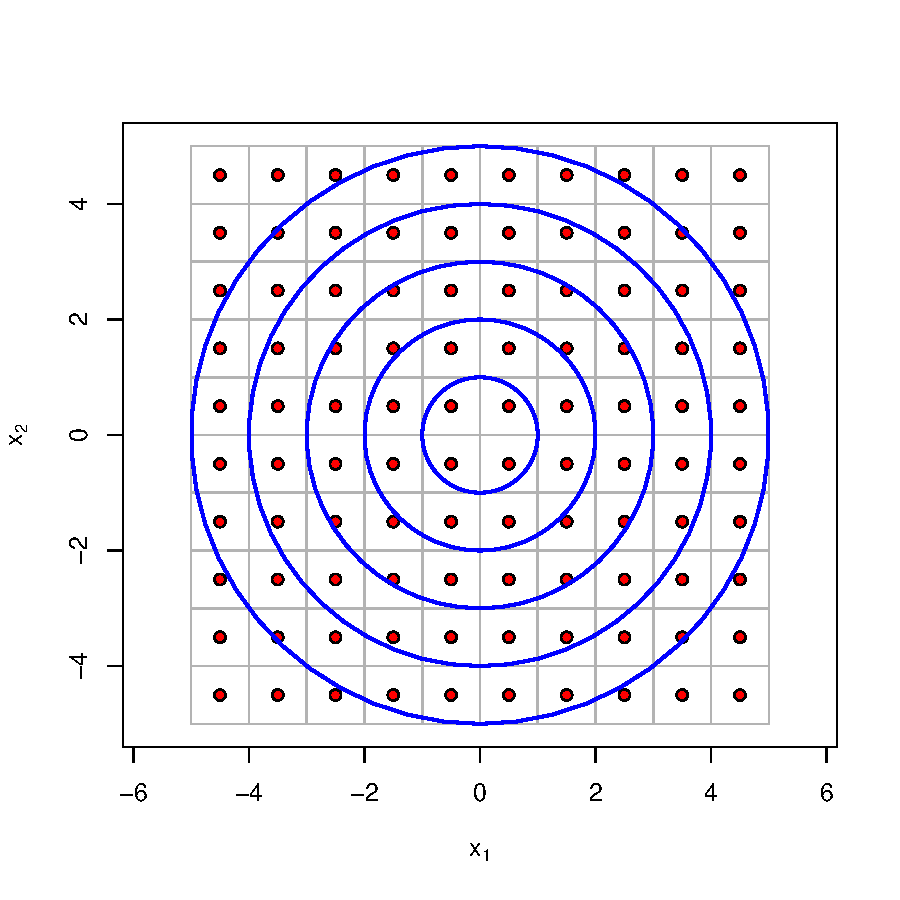
\includegraphics[scale=0.55]{original-contours.pdf}
\raisebox{4.0cm}{$\quad\xrightarrow{\vec{y}=A\vec{x}+\vec{\mu}}\quad$}
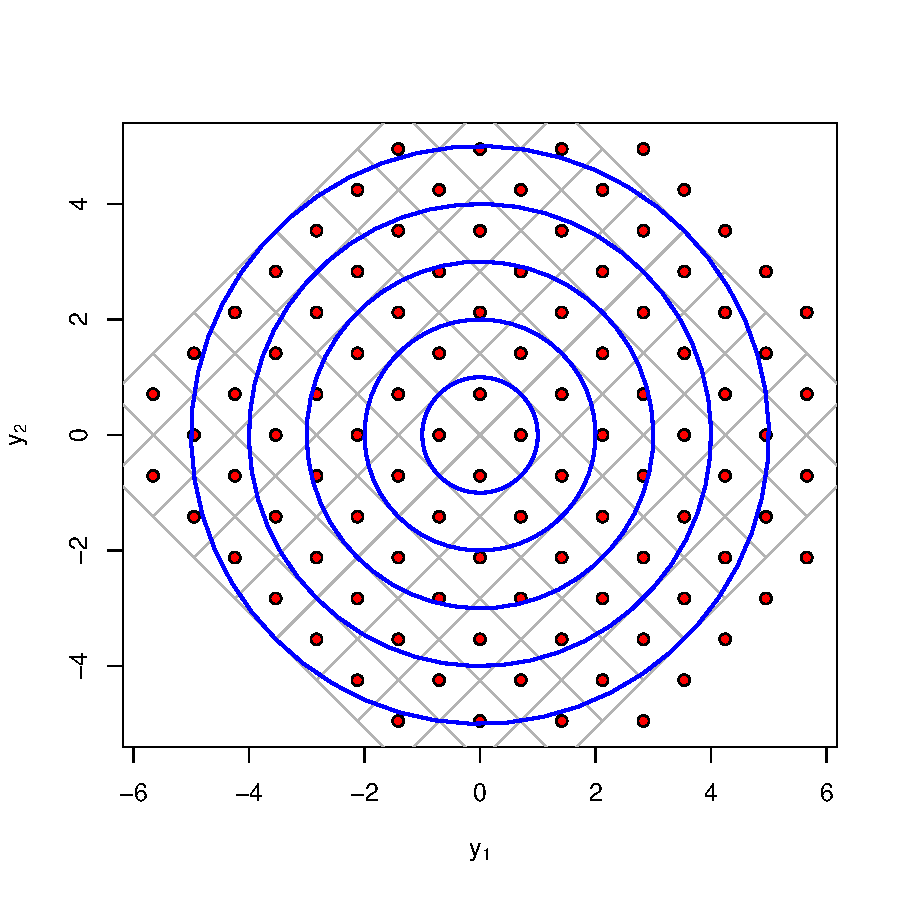
\includegraphics[scale=0.55]{rotated-contours.pdf}
\end{center}\vspace*{-1cm}



\foilhead[-1cm]{Simplified distribution reconstruction task}

\textbf{Achievable goal.}
Given the set of observations $\vec{y}_1,\ldots, \vec{y}_m$ determine the affine transformation by fixing the centre and axis of the ellipsoid.


\begin{center}
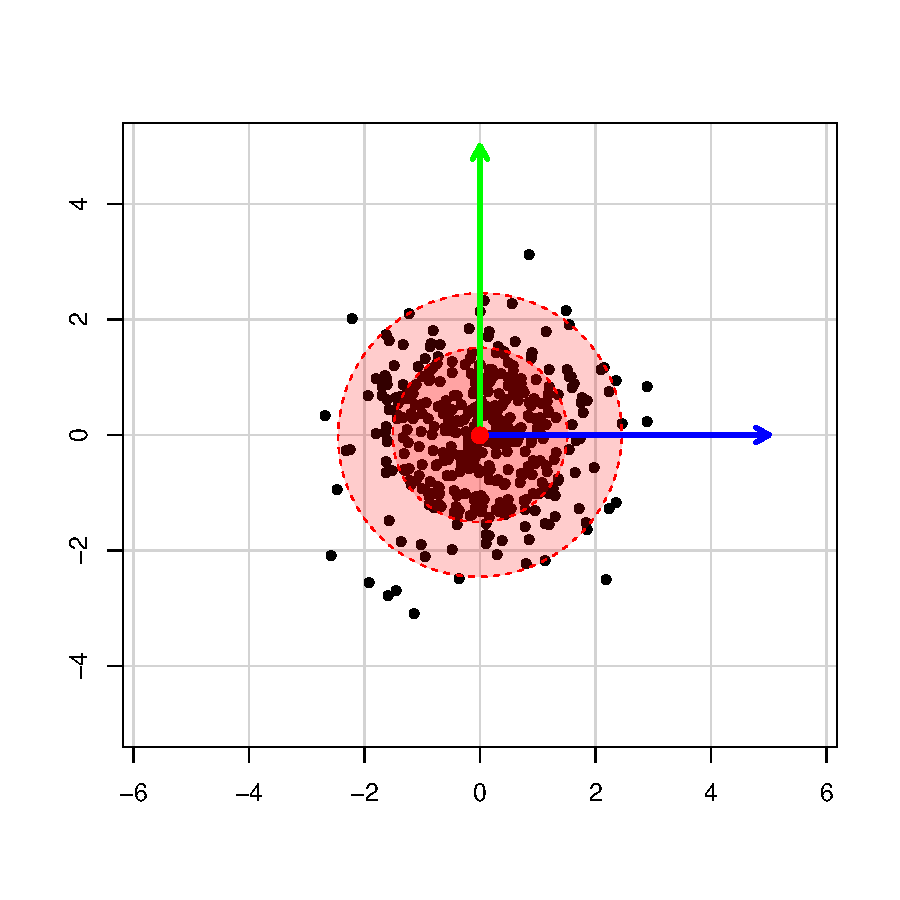
\includegraphics[scale=0.55]{source-distribution-iii.pdf}
\raisebox{4.0cm}{$\quad\xrightarrow{\vec{y}=A\vec{x}+\vec{\mu}}\quad$}
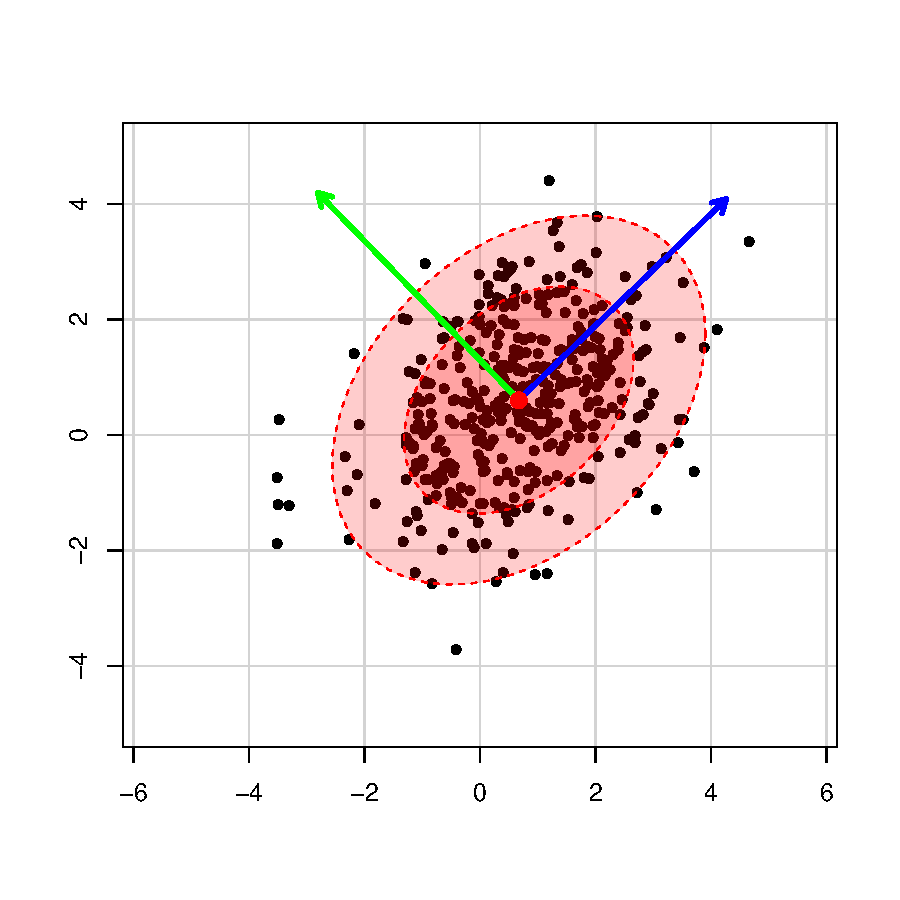
\includegraphics[scale=0.55]{target-distribution-iii.pdf}
\end{center}\vspace*{-1cm}

\begin{triangles}
\item We need to find the origin and semi-axes $\vec{a}_1,\ldots,\vec{a}_n$ of the ellipsoid.
\item Unit vectors $\vec{e}_1,\ldots,\vec{e}_n$ are mapped to semi-axes $\vec{a}_1,\ldots,\vec{a}_n$ of ellipsoid.
\end{triangles}


\foilhead[-1cm]{Variance for a fixed direction}

\textbf{Fact.} Ortogonal projection onto a unit vector $\vec{w}$  is given by scalar product.\vspace*{0.5cm}

\textbf{Question.} What is the direction $\vec{w}$ that maximises the variance for ellipsoid?
\begin{align*}
\VAR(\vec{w}^T \diag(\vec{a})\vec{x})=\VAR\Biggl(\sum_{i=1}^n w_i a_i x_i\Biggr)= \sum_{i=1}^n w_i^2 a_i^2\enspace. 
\end{align*}
The variance is maximised in the direction of the longest ellipse axis $a_1$. \vspace*{0.5cm}


\textbf{Question.}
How is the center of the ellipsoid and mean values connected?
\begin{align*}
\EXP(A\vec{x}+\vec{\mu})=\EXP(A\vec{x})+\EXP(\vec{\mu})= \vec{\mu}\enspace. 
\end{align*}


\foilhead[-1cm]{Principal component analysis}

\begin{triangles}
\item Compute the average value of the observations $\vec{y}_1,\ldots,\vec{y}_m$: 
\begin{align*}
\hat{\vec{\mu}}\gets\frac{\vec{y}_1+\cdots+\vec{y}_m}{m}\enspace.
\end{align*}
\item Centre the data by substituting $\hat{\vec{\mu}}$:
\begin{align*}
\vec{y}_i\gets \vec{y}_i-\hat{\vec{\mu}},\qquad i\in\set{1,\ldots,m}\enspace.
\end{align*}
\item Find the unit direction $\vec{w}_1$ that has \emph{a maximal empirical} variance: 
\begin{align*}
F(\vec{w})=\VAR(\vec{w}^T\vec{y}_1,\ldots,\vec{w}^T\vec{y}_n)=\frac{(\vec{w}^T\vec{y}_1)^2+\cdots+ (\vec{w}^T\vec{y}_m)^2}{m}\enspace.
\end{align*}
\item Find unit directions $\vec{w}_i$ orthogonal to previous directions that maximise the empirical variance of the corresponding the projection onto $\vec{w}_i$.  
\end{triangles}

\foilhead[-1cm]{Covariance matrix and optimisation goal}

We can use matrix algebra to simplify the variance estimate
\begin{align*}
F(\vec{w})&=\frac{1}{m}\cdot\Bigl(\vec{w}^T\vec{y}_1\vec{y}_1^T\vec{w}+\cdots+ \vec{w}^T\vec{y}_m\vec{y}_m^T\vec{w}\Bigr)\\
&=\vec{w}^T\biggl(\frac{\vec{y}_1\vec{y}_1^T+\cdots+\vec{y}_m\vec{y}_m^T}{m}\biggl)\vec{w}
\end{align*}
The $n\times n$ matrix in the middle is known as a \emph{covariance matrix} $\Sigma$.
\vspace*{1cm}

Due to the restriction $\norm{\vec{w}}_2^2=\vec{w}^T\vec{w}=1$, we have to use Lagrange' trick: 
\begin{align*}
F_*(\vec{w})&=\vec{w}^T\Sigma\vec{w}-2\lambda\vec{w}^T\vec{w}
\qquad \Rightarrow\qquad 
\frac{\partial F_*(\vec{w})}{\partial \vec{w}}=2\Sigma\vec{w}- 2\lambda\vec{w}=\vec{0}.
\end{align*}

\foilhead[-1cm]{Principal components as eigenvectors}

The $F_*(\vec{w})$ is maximised only if the direction $\vec{w}$ is an \emph{eigenvector} of $\Sigma$:
\begin{align*}
\Sigma\vec{w}=\lambda\vec{w}\qquad\Rightarrow\qquad \vec{w}^T\Sigma\vec{w}=\vec{w}^T\lambda\vec{w}=\lambda\enspace.
\end{align*}

\textbf{Fact.} If $n\times n$ matrix is symmetric and positively definite then there exists 
$n$ orthogonal eigenvectors $\vec{w}_1,\ldots,\vec{w}_n$ with \emph{eigenvalues} $\lambda_1\geq \ldots\geq\lambda_n>0$. \vspace*{0.5cm}

\textbf{Corollary.} Principal components corresponding to observations $\vec{y}_1,\ldots,\vec{y}_m$ are the eigenvectors of the covariance matrix $\Sigma$. 


\foilhead[-1cm]{Principal component analysis as a rotation}

Reconstruction of the source signal can be viewed as a \emph{translation} followed by a \emph{rotation} to orientate the ellipsoid wrt coordinate axis.

\begin{center}
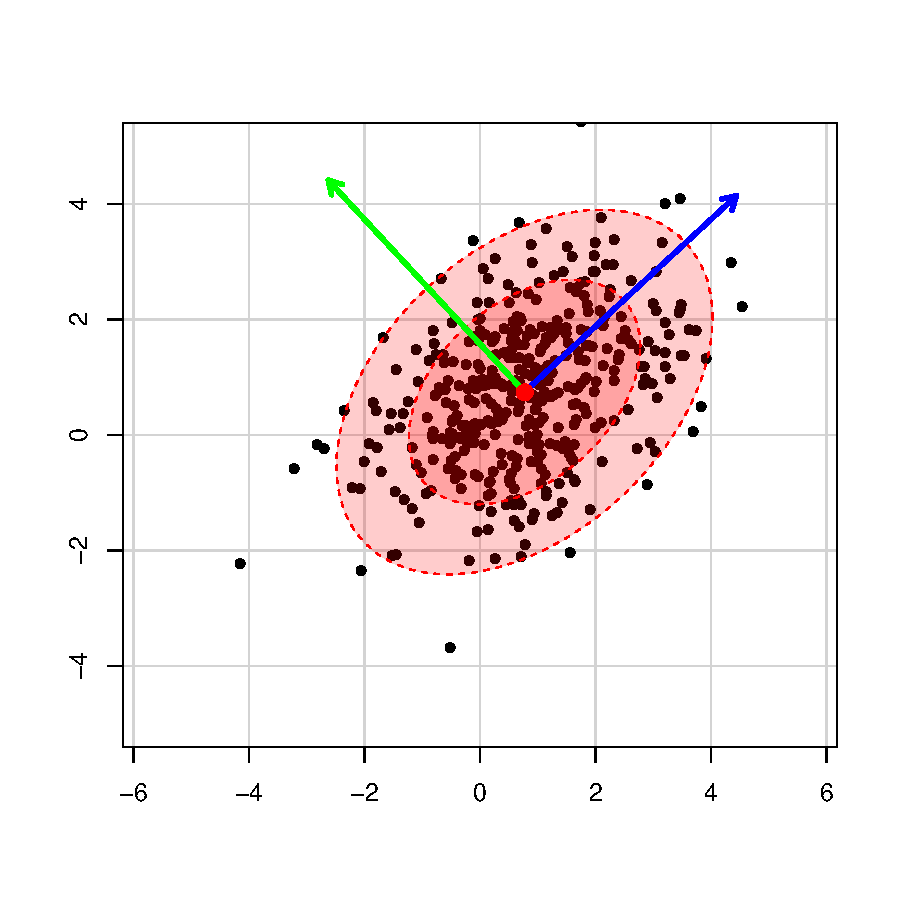
\includegraphics[scale=0.45]{initial-distribution-ii.pdf}
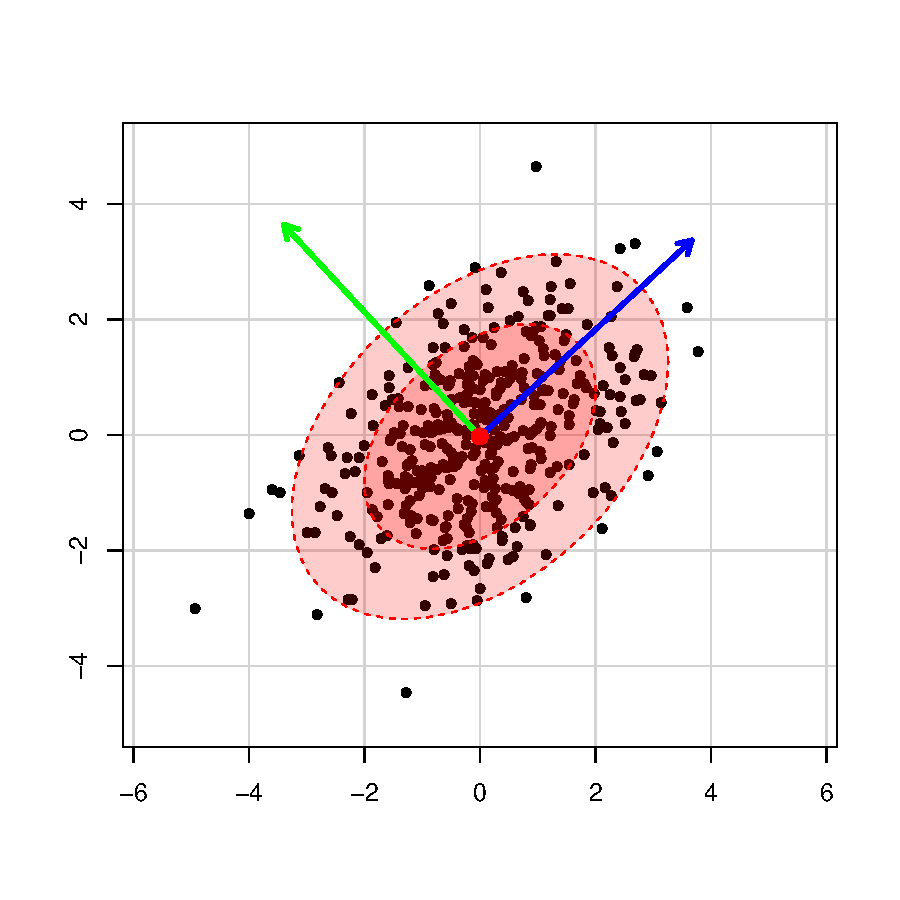
\includegraphics[scale=0.45]{translated-distribution-ii.pdf}
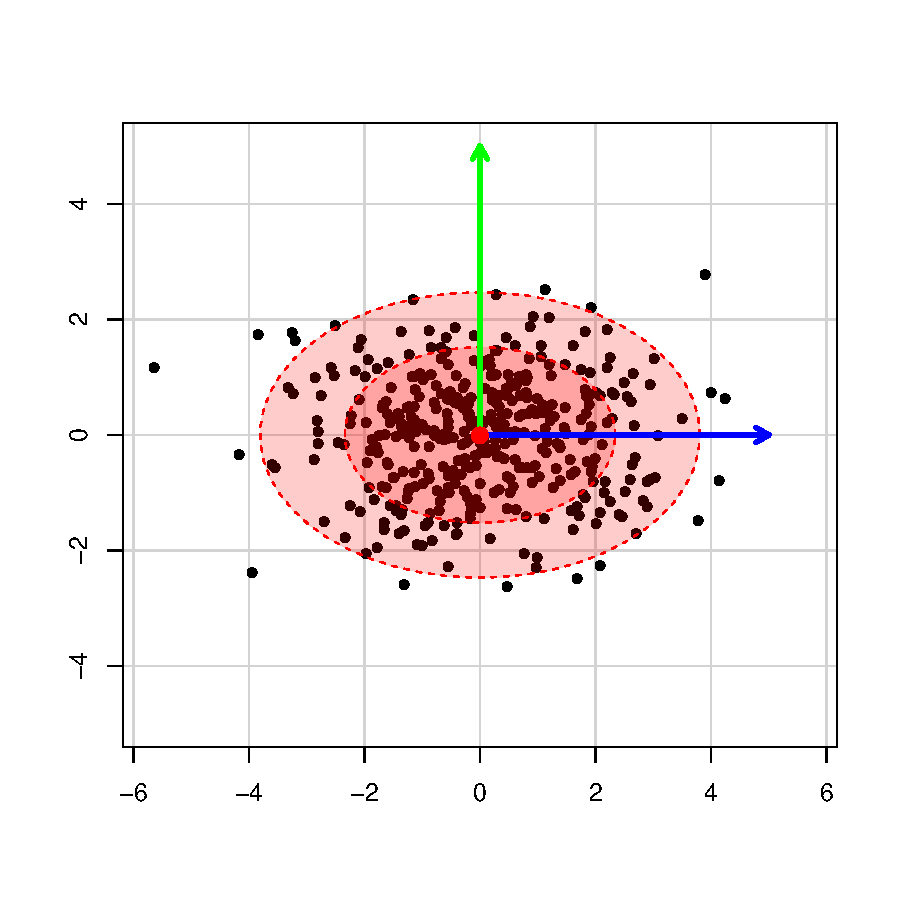
\includegraphics[scale=0.45]{rotated-distribution-ii.pdf}
\end{center}\vspace*{-1cm}

As vectors $\vec{w}_1,\ldots,\vec{w}_n$ are orthogonal, the rotation can be done through computing projections (read scalar products):
\begin{align*}
\hat{\vec{x}}_i= (\vec{w}_1 ||\cdots|| \vec{w}_n)^T (\vec{y}_i-\hat{\vec{\mu}}_0)=W(\vec{y}_i-\hat{\vec{\mu}})\enspace.
\end{align*}  


\foilhead[-1cm]{Maximum likelihood estimate}

The algorithm formulated above was based on \emph{ad hoc} reasoning:
\begin{triangles}
\item Empirical estimates for the mean and variance are not precise!
\end{triangles}\vspace*{1.5cm}

Theoretically correct way to handle the problem is
\begin{triangles}
\item obtain the maximum likelihood estimate on the model parameters,
\item determine the translation and rotation based on the model parameters.
\end{triangles}\vspace*{1.5cm}

What are the model parameters?
\begin{triangles}
\item Parameters of the density formula $\Sigma$ and $\vec{\mu}$.
\item Parameters of the affine transformation $A$ and $\vec{\mu}$.
\end{triangles}

\foilhead[-1cm]{Likelihood function under iid assumption}
If all observations $\vec{y}_1,\ldots,\vec{y}_m$ are independent then\vspace*{-0ex}
\begin{align*}
p[\vec{y}_i,\ldots,\vec{y}_m|\Sigma,\vec{\mu}]
&=\prod_{i=1}^m p[\vec{y}_i|\Sigma,\vec{\mu}]
\end{align*}\vspace*{-4ex}\\
where\vspace*{-0ex}
\begin{align*}
p[\vec{y}_i|\Sigma,\vec{\mu}]
&=\frac{1}{(2\pi)^{n/2}}\cdot\frac{1}{\sqrt{\det(\Sigma)}}\cdot
\exp{-\frac{(\vec{y}_i-\vec{\mu})^T \Sigma^{-1}(\vec{y}_i-\vec{\mu})}{2}}\enspace
\end{align*}\vspace*{-0ex}\\
The \emph{log-likelihood} of the data $\ln p[\vec{y}_i,\ldots,\vec{y}_m|\Sigma,\vec{\mu}]$ can be expressed \vspace*{-0ex}
\begin{align*}
\LLL(\Sigma,\vec{\mu})=const +\frac{m}{2}\cdot \ln\det(\Sigma^{-1}) 
-\sum_{i=1}^m\frac{(\vec{y}_i-\vec{\mu})^T \Sigma^{-1}(\vec{y}_i-\vec{\mu})}{2}
\end{align*}
Now we have to find the arrangement $(\Sigma,\vec{\mu})$ that maximises $\LLL(\Sigma,\vec{\mu})$.\lastline
 
\foilhead[-1cm]{Gradients of the log-likelihood function}

Gradient with respect to the shift $\vec{\mu}$: 
\begin{align*}
\frac{\partial\LLL}{\partial\vec{\mu}}= -\sum_{i=1}^m\frac{\partial}{\partial\vec{\mu}}\frac{(\vec{y}_i-\vec{\mu})^T \Sigma^{-1}(\vec{y}_i-\vec{\mu})}{2}
=-\sum_{i=1}^m\frac{\Sigma^{-1}(\vec{y}_i-\vec{\mu})}{2}\cdot(-1)
\end{align*}
Gradient with respect to the inverse matrix $\Sigma^{-1}$: 
\begin{align*}
\frac{\partial\LLL}{\partial(\Sigma^{-1})}&=\frac{m}{2}\cdot \frac{\partial}{\partial(\Sigma^{-1})} \ln\det(\Sigma^{-1}) -\sum_{i=1}^m\frac{\partial}{\partial(\Sigma^{-1})}\frac{(\vec{y}_i-\vec{\mu})^T \Sigma^{-1}(\vec{y}_i-\vec{\mu})}{2}\\
&=\frac{m}{2}\cdot\Sigma^{T} -\sum_{i=1}^m\frac{(\vec{y}_i-\vec{\mu})^T (\vec{y}_i-\vec{\mu})}{2}
\end{align*}
As $\Sigma$ is symmetric and $\Sigma^{-1}$ exists we can derive closed form solutions.

\foilhead[-1cm]{Maximum likelihood estimates for parameters}

The shift must be the mean of all observations
\begin{align*}
\vec{\mu}=\frac{1}{m}\cdot \sum_{i=1}^m\vec{y}_i\enspace.
\end{align*} 
The covariance matrix 
\begin{align*}
\Sigma=\frac{1}{m}\cdot\sum_{i=1}^m(\vec{y}_i-\vec{\mu})^T (\vec{y}_i-\vec{\mu})
\end{align*}

\textbf{Correctness of PCA.}
As ML estimates are exactly the same  we used in principal component analysis, the method is theoretically justified!\lastline


\middlefoil{Principal component analysis\vspace*{1ex}\\
 {Alternative formalisations}}

\foilhead[-1cm]{Dimensionality reduction}

What if the actual data $\vec{x}_1,\ldots,\vec{x}_m$ lies in a lower-dimensional plane and the observation  $\vec{y}_1,\ldots,\vec{y}_m$ are obtained by random shifts?   



\begin{center}
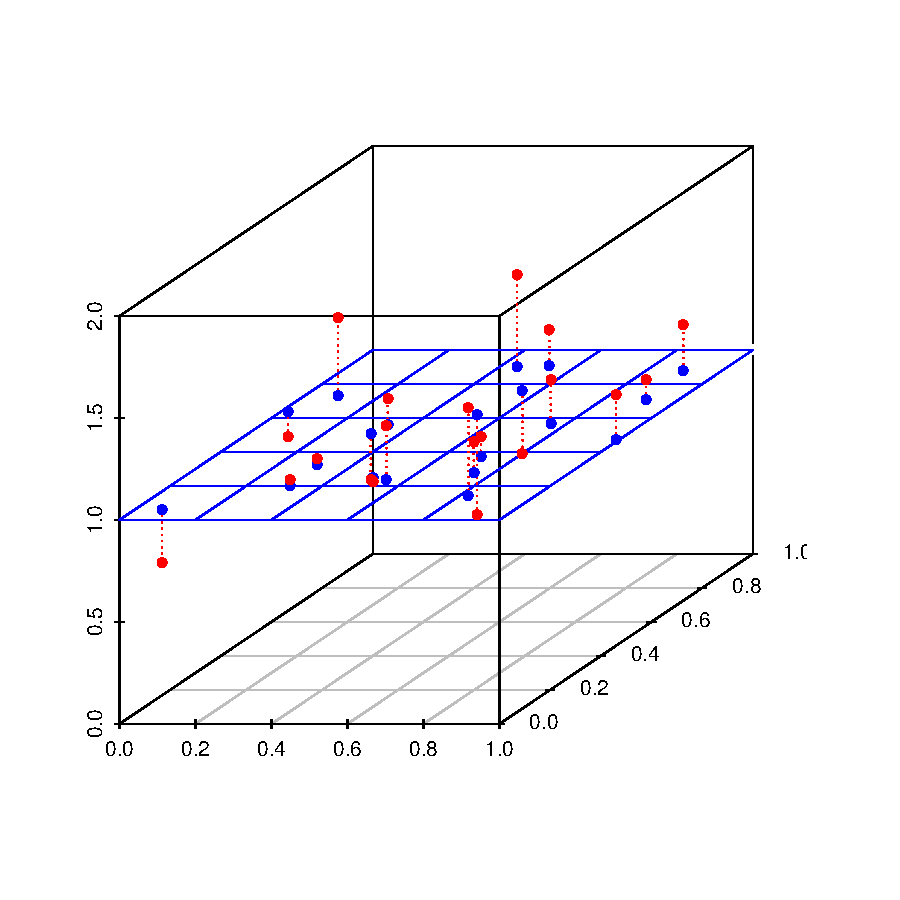
\includegraphics[scale=0.55]{low-dimensional-data-i.pdf}
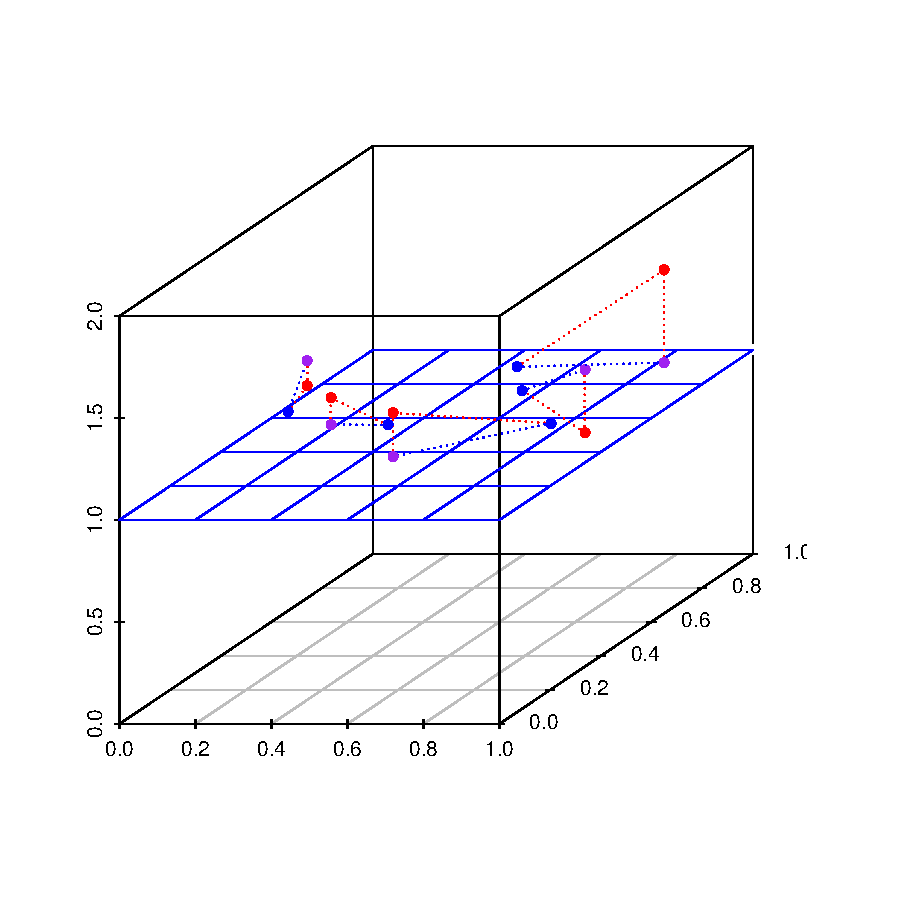
\includegraphics[scale=0.55]{low-dimensional-data-ii.pdf}
\end{center}\vspace*{-1cm}

The shifts can be either orthogonal to the plane or just random. The first model is easier to analyse while the second is more plausible. 


\foilhead[-1cm]{Maximum likelihood estimate}

Let $\HHH$ be the plane. Assume that the random shifts $\varepsilon_i$ are orthogonal to the plane and have a normal distribution $\NNN(0,\sigma I)$. Then 
\begin{align*}
p[\vec{y}_i|\HHH,\sigma]=const\cdot\exp{-\frac{d_i^2}{2\sigma^2}}
\end{align*}
where $d_i$ is the distance between the plane $\HHH$ and the point $\vec{y}_i$. Thus
\begin{align*}
p[\vec{y}_1,\ldots,\vec{y}_m|\HHH,\sigma]=const\cdot\exp{-\sum_{i=1}^m\frac{d_i^2}{2\sigma^2}}
\end{align*}
and the maximum likelihood estimate of the plane minimises sum of the distance squares. Corresponding estimates of $\vec{x}_1,\ldots,\vec{x}_m$ are projections of $\vec{y}_1,\ldots,\vec{y}_m$ to the plane $\HHH$.\lastline 

\foilhead[-1cm]{Another characterisation of PCA}

\textbf{Fact.} If the data is centred then PCA chooses the direction $\vec{w}_1$ such that
the sum of squares of the projections $\vec{w}_1^T \vec{y}_i$ is maximal.\vspace*{-1cm}

\begin{center}
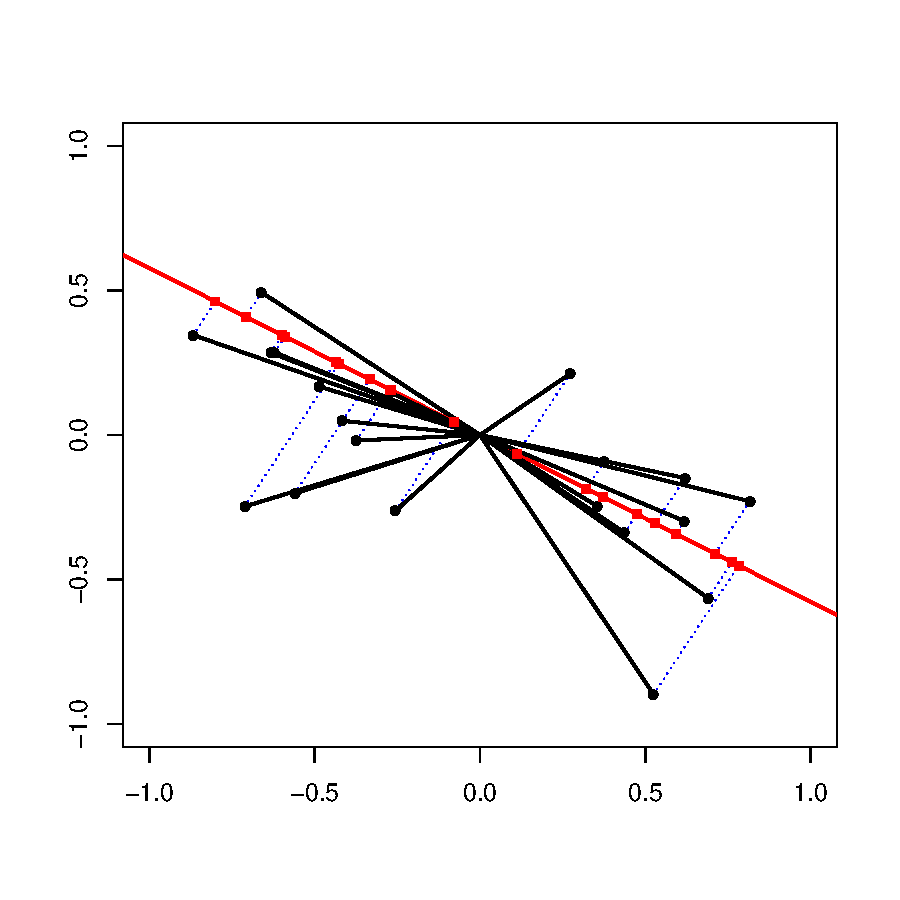
\includegraphics[scale=0.65]{orthogonal-projection.pdf}
\end{center}\vspace*{-1cm}


\textbf{Corollary.} PCA chooses directions $\vec{w}_1,\ldots,\vec{w}_n$ such that the sum of distance squares from the hyperplane formed by $\vec{w}_1,\ldots,\vec{w}_k$ is minimal. 

\foilhead[-1cm]{PCA as a dimensionality reduction tool}

\textbf{Corollary.} PCA rotates the data such way that first $k$ coordinates of the rotated data correspond to maximum likelihood reconstructions of original vectors corrupted with white Gaussian noise $\NNN(0,\sigma I)$.  


\begin{center}
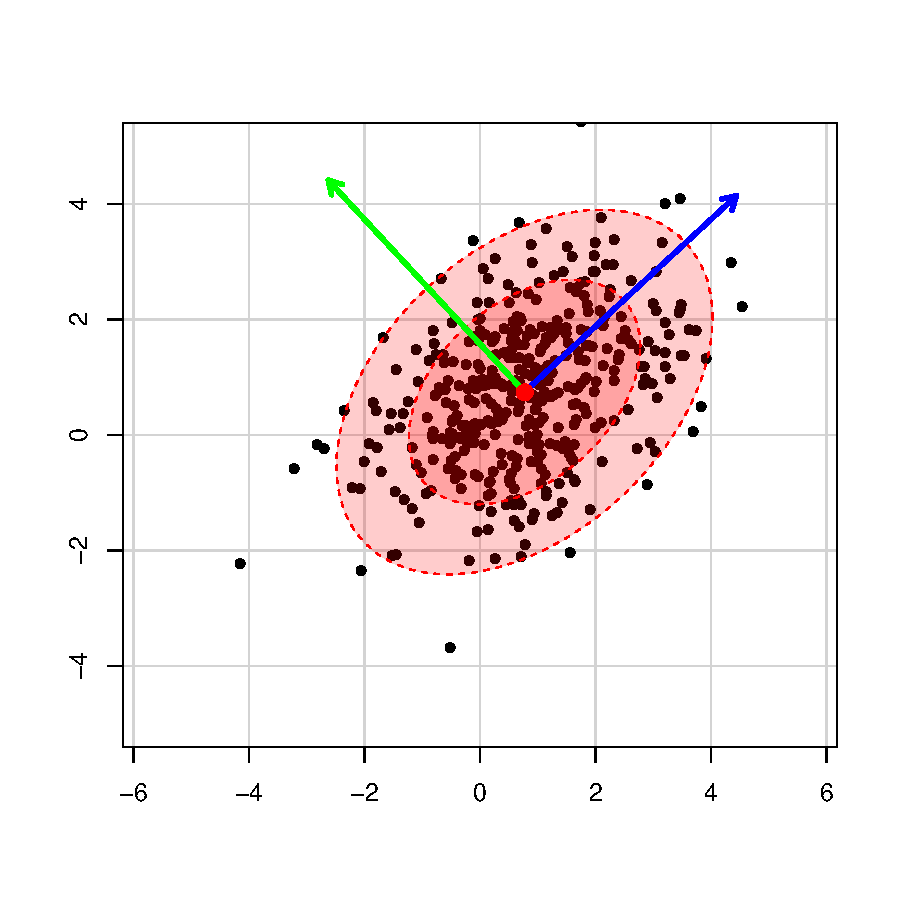
\includegraphics[scale=0.45]{initial-distribution-ii.pdf}
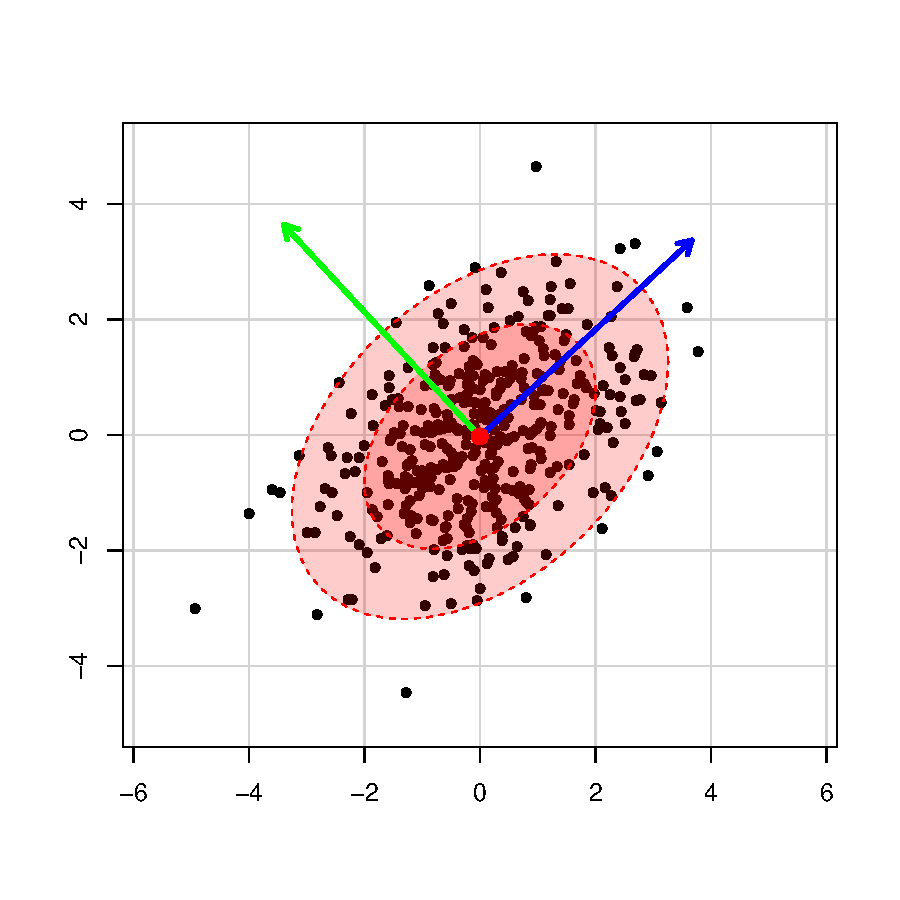
\includegraphics[scale=0.45]{translated-distribution-ii.pdf}
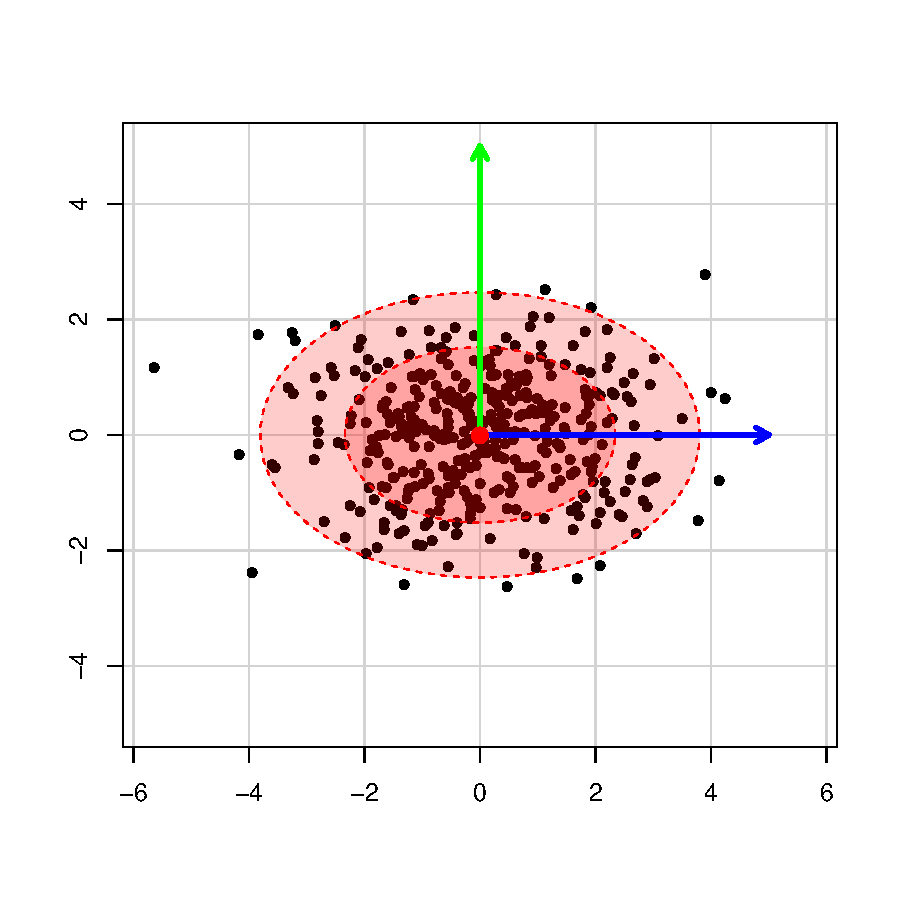
\includegraphics[scale=0.45]{rotated-distribution-ii.pdf}
\end{center}\vspace*{-1cm}

Alternatively, we can view the last components of the source signal $\vec{x}$ as the uninformative noise. The overall noise component should be small.\lastline

\foilhead[-1cm]{Connection to autoencoders}

\begin{tabular}{cc}
Linear autonecoder & RELU autoencoder\\

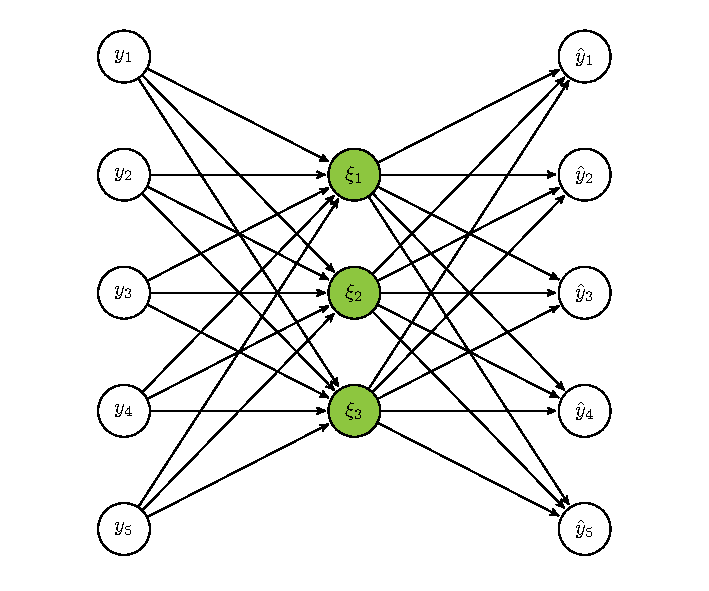
\includegraphics[scale=0.8]{linear-autoencoder}
&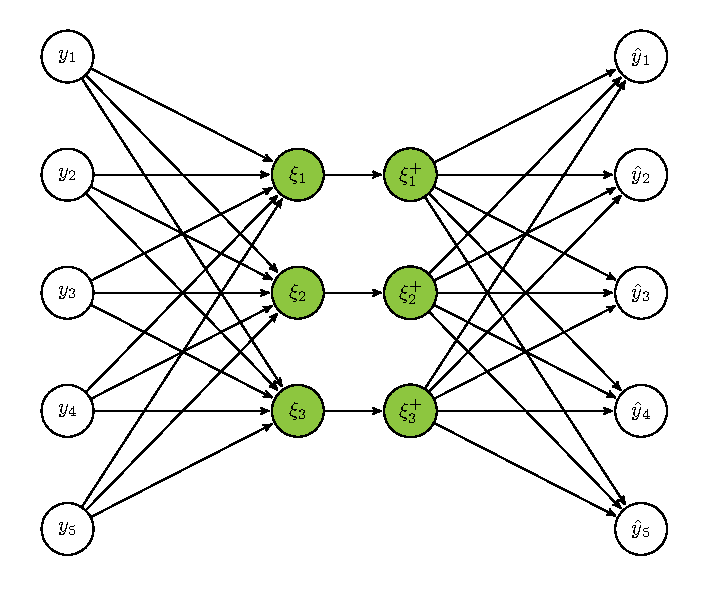
\includegraphics[scale=0.8]{relu-autoencoder}\\
\end{tabular}

Fix mean square error as optimisation target. %\vspace*{-1ex}
\begin{triangles}
\item Linear-autoencoder is a reformulation of PCA.  
\item RELU-autoencoder is a reformulation of non-negative matrix~factorisation.
\end{triangles}



\foilhead[-1cm]{Connection to convolutional neural networks}

\begin{tabular}{cc}
Hierarchical NMF & Convolutional network\\

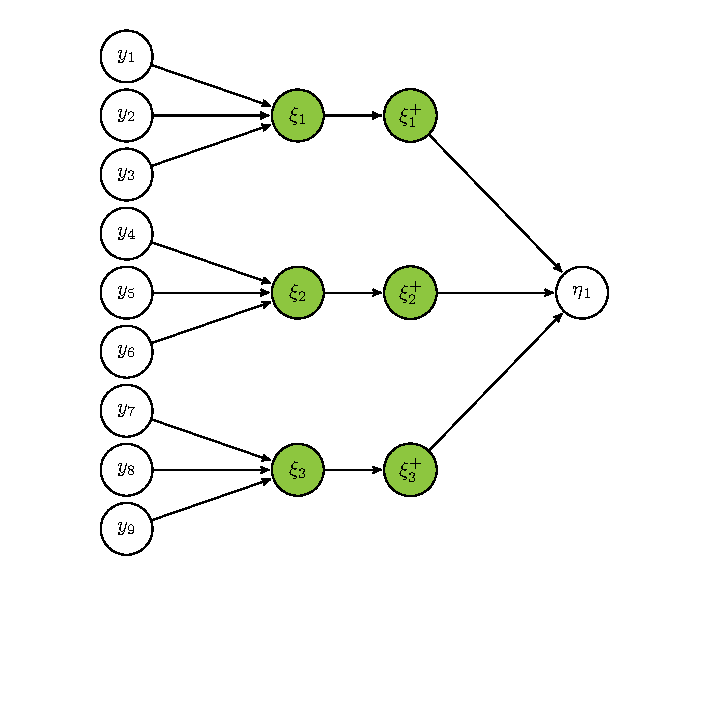
\includegraphics[scale=0.7]{hierarchical-nmf}
&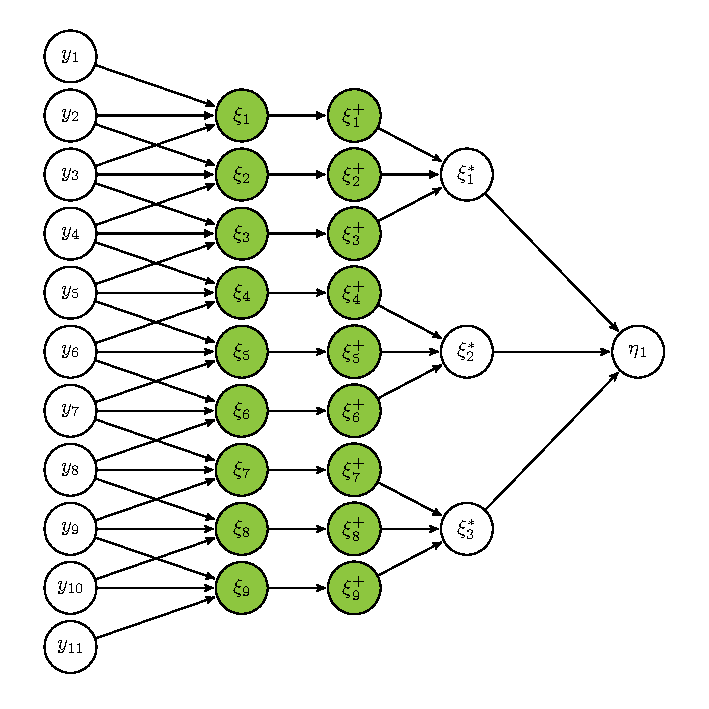
\includegraphics[scale=0.7]{convolutional-network}\\
\end{tabular}

\begin{triangles}
\item Hierarchical NMF applies the same transformation on patches.
\item Convolutional layer applies the same transformation to sliding windows.
\item Then it picks the strongest response among shifts of the transformation.
\end{triangles}



\middlefoil{Linear discriminant\vspace*{1ex}\\ analysis}

\foilhead[-1cm]{Underlying assumptions and inference task}

\textbf{Original goal.}
Given a set of observations $\vec{x}_1,\ldots,\vec{x}_n\in\RR^M$ together with class labels $z_1,\ldots,z_n\in\set{1,\ldots,\ell}$ find a linear projection $\pi:\RR^m\to\RR^k$ so that individual classes are maximally separated.\vspace*{1cm}

\textbf{Assumptions.}
\begin{triangles}
\item There are $\ell$ different classes. 
\item All observations $\vec{x}_i$ are independently sampled.
\item Observations $\vec{x}_i$ with the same class label $z_i$ come from $\NNN(\vec{\mu}_j, \Sigma)$.
\item The covariance matrix $\Sigma$ is shared between different distributions.
\end{triangles}

\foilhead[-1cm]{LDA for spherical normal distributions}

\illustration[scale=0.5]{simplified_lda_setup_i}

We assume that the covariance matrix $\Sigma$ is identity matrix: 
\begin{triangles}
\item All vector components have unit variance. 
\item Different vector components are independent.
\end{triangles}

\foilhead[-1cm]{Projections to one-dimensional subspace}

\illustration[scale=0.5]{simplified_lda_setup_ii}

A projection to one-dimensional space is determined by a vector $\vec{w}$:
\begin{triangles}
\item To get orthogonal projection the length of $\vec{w}$ must be one.
\item This can be forced by the constraint $\vec{w}^T\vec{w}=1$.  
\end{triangles}

\foilhead[-1cm]{Projections lead to different separation}

\illustration[scale=0.7]{simplified_lda_setup_iii}

We need a need a  measure for assessing the goodness of separation: 
\begin{triangles}
\item We can use Bayesian factors from statistics.
\item We can use signal-to-noise ratio from signal-processing.
\end{triangles}

\foilhead[-1cm]{Choice between alternative hypotheses}

\begin{triangles}
\item \textbf{Hypothesis $\HHH_0$.} Projections $y_i,\ldots, y_n$ come from $\mathcal{N}(\bar{y}, 1)$.
\item \textbf{Hypothesis $\HHH_1$.} Projection $y_i$ with label $z_i$ comes from a $\mathcal{N}(\bar{y}_{z_i},1)$.\vspace*{2ex}
\end{triangles}

Hypotheses lead to following probability assignments
\begin{align*}
p[y_i|\HHH_0]&=\frac{1}{\sqrt{2\pi}}\cdot \exp{-\frac{1}{2}(y_i-\bar{y})^2}\\
p[y_i|\HHH_1]&=\frac{1}{\sqrt{2\pi}}\cdot \exp{-\frac{1}{2}(y_i-\bar{y}_{z_i})^2}
\end{align*}
If we have not preference then the corresponding Bayes factor is
\begin{align*}
\frac{\Pr[\HHH_1|y_1,\ldots,y_n]}{\Pr[\HHH_0|y_1,\ldots,y_n]}= 
\exp{\frac{1}{2}\cdot\sum_{i=1}^n(y_i-\bar{y})^2-\frac{1}{2}\cdot\sum_{i=1}^n(y_i-\bar{y}_{z_i})^2}
\end{align*}

\foilhead[-1cm]{The corresponding optimisation task}

Given a set of observations $\vec{x}_1,\ldots,\vec{x}_n\in\RR^M$ together with class labels $z_1,\ldots,z_n\in\set{1,\ldots,\ell}$ find a vector $\vec{w}$ with unit length that maximises:
\begin{align*}
F=\sum_{i=1}^n(y_i-\bar{y})^2-\sum_{i=1}^n(y_i-\bar{y}_{z_i})^2\enspace
\end{align*}
where $\mathcal{I}_j=\set{i: z_i=j}$ is the index set and $\bar{y}$ and $\bar{y}_{j}$ are cluster means: 
\begin{align*}
\bar{y}&=\frac{1}{n}\cdot\sum_{i=1}^n y_i \\
\bar{y}_j&=\frac{1}{|\mathcal{I}_j|}\cdot\sum_{i\in\mathcal{I}_j} y_j 
\end{align*}

\foilhead[-1cm]{Consequences of variance decomposition}

Given a set of observations $\vec{x}_1,\ldots,\vec{x}_n\in\RR^M$ together with class labels $z_1,\ldots,z_n\in\set{1,\ldots,\ell}$ find a vector $\vec{w}$ with unit length that maximises:
\begin{align*}
F=\sum_{i=1}^n(\bar{y}_{z_i}-\bar{y})^2\enspace
\end{align*}

\textsc{Proof.}
The result follows directly form the variance decomposition
\begin{align*}
\sum_{i=1}^n (y_i-\bar{y})^2
&=\sum_{i=1}^n (y_i-\bar{y}_{z_i})^2 +\sum_{i=1}^n (\bar{y}_{z_i}-\bar{y})^2
\end{align*}



\foilhead[-1cm]{Matrix magic}

Let us define centres in the original data 
\begin{align*}
\vec{\mu}&=\frac{1}{n}\cdot\sum_{i=1}^n \vec{x}_i &
\vec{\mu}_j&=\frac{1}{|\mathcal{I}_j|}\cdot\sum_{i\in\mathcal{I}_j}^n \vec{x}_j
\end{align*}
Then we can express
\begin{align*}
F&=\sum_{i=1}^n(\bar{y}_{z_i}-\bar{y})^2\enspace
=\sum_{i=1}^n(\vec{w}^T\vec{\mu}_{z_i}-\vec{w}^T\vec{\mu})(\vec{w}^T\vec{\mu}_{z_i}-\vec{w}^T\vec{\mu})^T\\
&=\vec{w}^T\Biggl(\sum_{i=1}^n(\vec{\mu}_{z_i}-\vec{\mu})(\vec{\mu}_{z_i}-\vec{\mu})^T\Biggr)\vec{w}
\end{align*}

\foilhead[-1cm]{Corresponding eigenvector task}

Find a vector $\vec{w}$ with unit length that maximises
\begin{align*}
F=\vec{w}^T S_B\vec{w}
\end{align*}
where $S_B$ is the between class scatter matrix;
\begin{align*}
S_B=\sum_{i=1}^n(\vec{\mu}_{z_i}-\vec{\mu})(\vec{\mu}_{z_i}-\vec{\mu})^T \enspace.
\end{align*} 

\textbf{Consequence.}
The function $F$ is maximised by the eigenvector $\vec{w}$ of $S_B$ with the highest eigenvalue $\lambda_1$.

\foilhead[-1cm]{LDA for a normal distribution with any shape}

\illustration[scale=0.75]{general_lda_setup_i}

\begin{triangles}
\item As we know cluster labels we can remove the effect of $\vec{\mu}_1,\ldots\vec{\mu}_\ell$.
\item After that we can do affine transformation that set the covariance to $I$.
\item We know how to solve the task in the transformed space. 
\end{triangles}

\foilhead[-1cm]{Data whitening transformation}

A linear transformation $\vec{x}^*=A\vec{x}$ leads to a unit covariance $I$ if 
\begin{align*}
A\Sigma_W A^T=I
\end{align*}  
where $\Sigma_W$ is within class covariance matrix:
\begin{align*}
\Sigma_W=\frac{1}{n}\cdot \sum_{i=1}^n (\vec{x}_i-\vec{\mu}_{z_i})(\vec{x}_i-\vec{\mu}_{z_i})^T
\end{align*}
Let $W$ be the matrix where column vectors $\vec{w}_i$ are orthonormal eigenvectors with eigenvalues $\lambda_1,\ldots,\lambda_n$. Then we can express 
\begin{align*}
A=\diag(\lambda_1^{-1/2},\ldots,\lambda_n^{-1/2})W^T\enspace. 
\end{align*} 

\foilhead[-1cm]{The effects of data whitening}

\centerline{
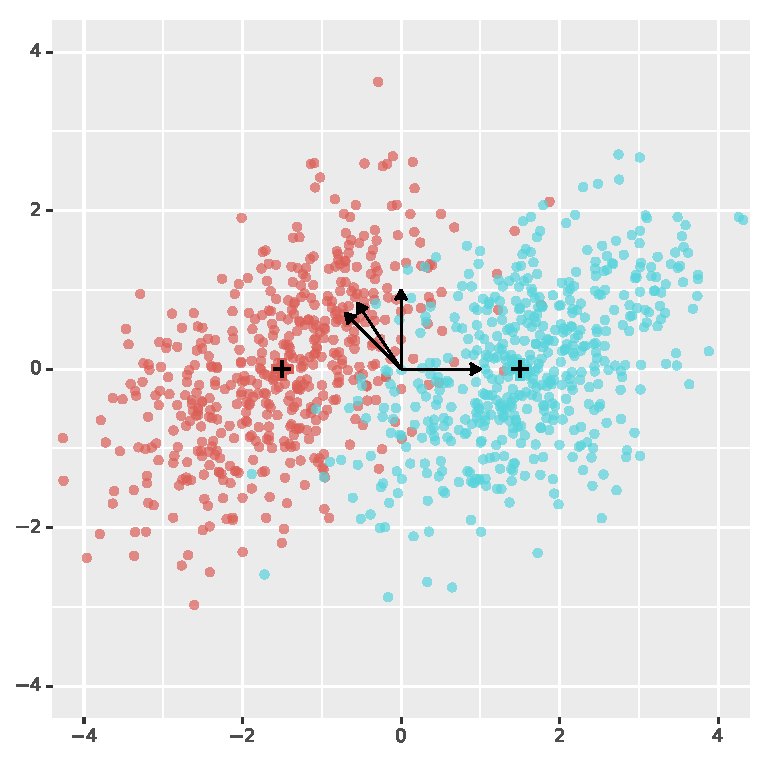
\includegraphics[scale=0.70]{general_lda_setup_ii}\hspace*{1cm}
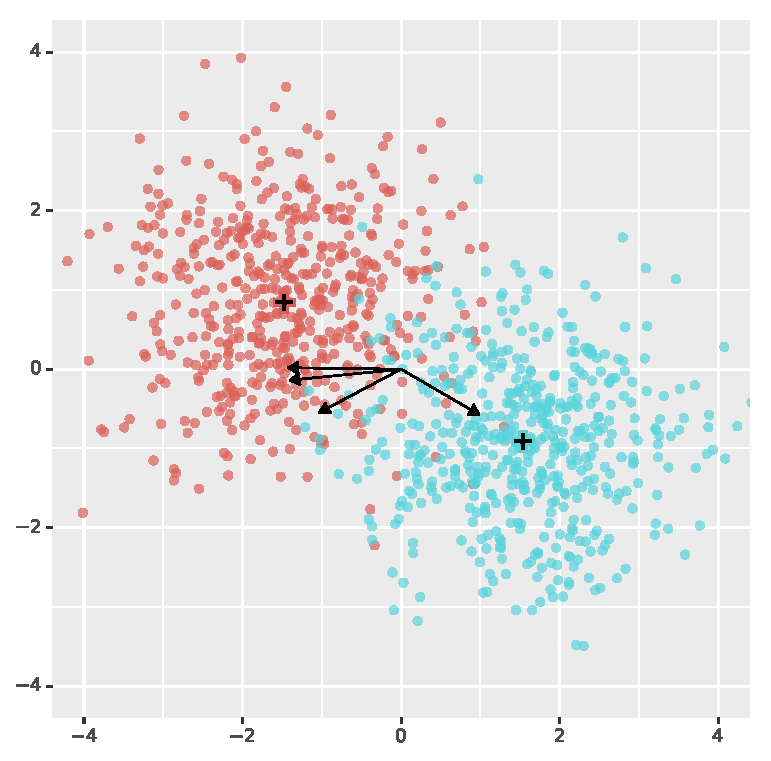
\includegraphics[scale=0.70]{general_lda_setup_iv}}\vspace*{-1ex}

\begin{triangles}
\item Data whitening alters probing directions: $\vec{w}^*=A\vec{w}$. 
\item Data whitening alters between class scatter: $S_B^*=AS_BA^T$. 
\item Maximisation task in original terms: $\sum_{i=1}^k\vec{w}_i^T\Sigma_W^{-T}S_B\Sigma_W^{-1}\vec{w}_i\to \max$
\item Othogonality constraints in original terms: $\vec{w}_i^T\Sigma_W^{-1}\vec{w}_j=\delta_{ij}$.\vspace*{-1cm}     
\end{triangles}

\foilhead[-1cm]{Numerical stabilisation}

Whitening matrix $\Sigma_W$ can be non-invertible and it can also depend heavily on the perturbations of original datapoints. Ridge stabilisation 
\begin{align*}
\Sigma_W^*=\Sigma_W+\rho I
\end{align*}   
for small value $\rho>0$ makes linear discriminant analysis more stable.

\foilhead[-1cm]{Connection to neural networks}

\begin{tabular}{cc}
Linear + SoftMax & RELU + SoftMax\\

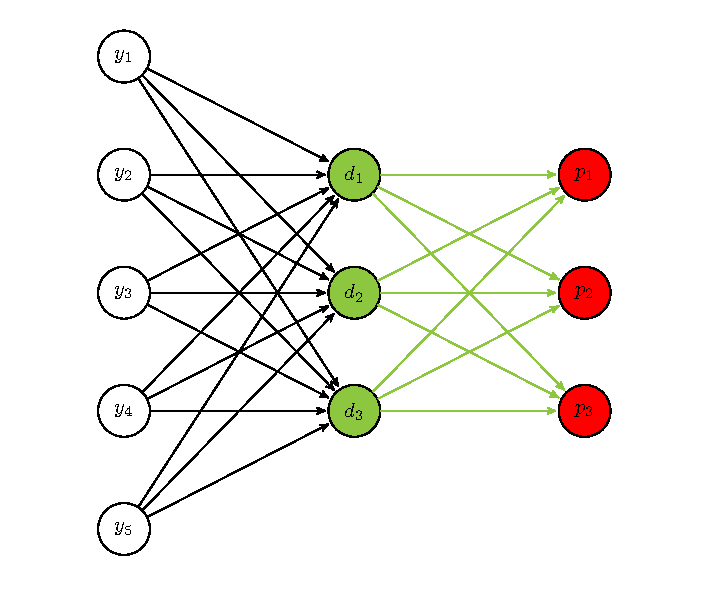
\includegraphics[scale=0.8]{linear-softmax-classifer}
&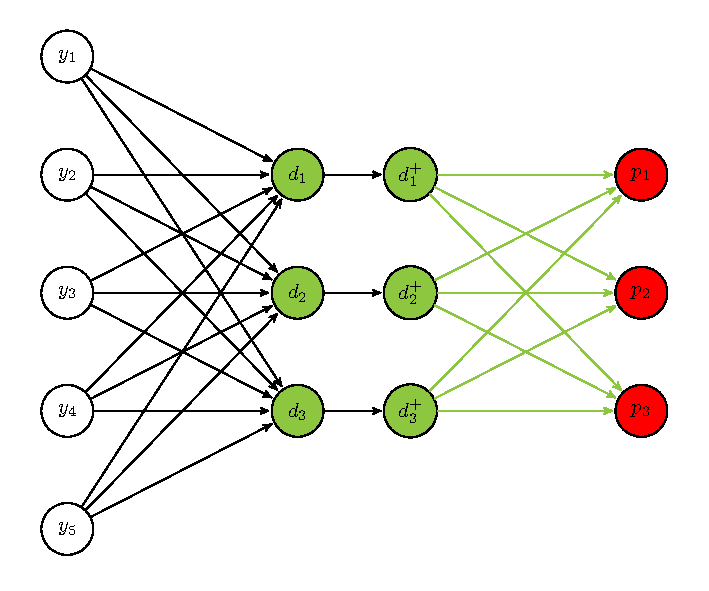
\includegraphics[scale=0.8]{relu-softmax-classifer}\\
\end{tabular}

\begin{triangles}
\item LDA is equivalent to a linear layer \mbox{followed~by~a~soft-max~layer.}
\item Neural networks usually use RELU nodes instead of pure linear nodes.   
\item This again introduces non-negativity constraint to features. 
\end{triangles}


\foilhead[-1cm]{Reconstruction vs discrimination}

\begin{triangles}
\item PCA and LDA reduce dimensionality.
\item PCA preserves recoverability of the original data.
\item LDA preserves distinguishability between different classes. \vspace*{1cm}     
\end{triangles}

Sometimes discriminative are overly selective:
\begin{triangles}
\item Decision is made based on minute details of the data
\item Predictions are not robust against malicious perturbations.\vspace*{1cm} 
\end{triangles}

We can quantify the balance between reconstruction vs discrimination. 
\begin{triangles}
\item We can measure how much variation LDA projection explains.
\item We can measure robustness against input perturbations. 
\item Same measures are applicable for other models such as neural networks.
\end{triangles} 




\middlefoil{Going beyond basics}


\foilhead[-1cm]{Going beyond PCA and LDA}

Weighted Principal Component Analysis:
\begin{triangles}
\item Sometimes data contains potential outliers.
\item Sometimes we can assign reliability scores to the data points. 
\end{triangles}\vspace*{1.0cm}

Principal curves and manifolds
\begin{triangles}
\item The original data might be on a low dimensional manifold. 
\item The observed data is corrupted by additive white gaussian noise. 
\item The task is to reconstruct the manifold and ML estimate for the data. 
\end{triangles}\vspace*{1.0cm}


Independent Component Analysis 
\begin{triangles}
\item What if the source components are non-gaussian? 
\item Then the reconstruction is possible up to scaling!
\end{triangles} 


\foilhead[-3cm]{Principal curves and manifolds}

\begin{center}
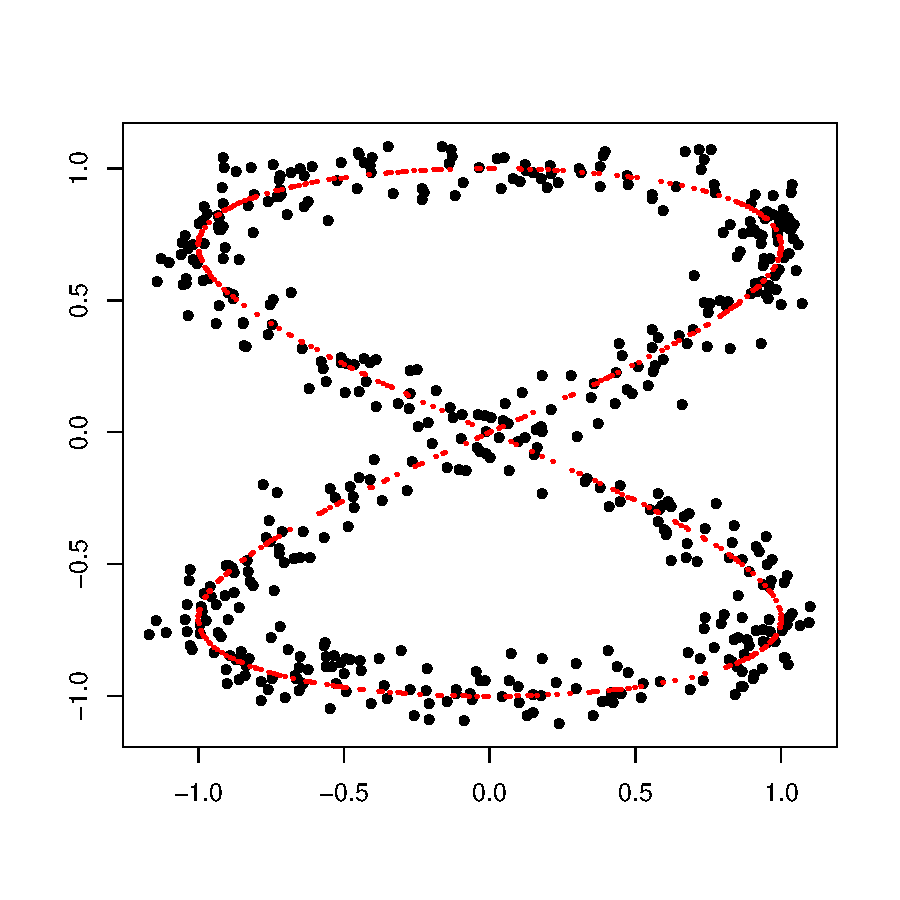
\includegraphics[scale=0.75]{principal-curve.pdf}
\end{center}\vspace*{-1cm}

Reconstruction of the underlying curve is much more difficult.
\begin{triangles}
\item We must fix a curve parametrisation 
\item The task is different form regression since we have only outputs.
\end{triangles} 
 


\foilhead[-1cm]{Independent Component Analysis}

Assume that the components of the source data $\vec{x}_1,\ldots,\vec{x}_m$ are independent  
but an unknown affine transformation  $\vec{y}=A\vec{x}+\vec{\mu}$ disturbs observations. 
\begin{center}
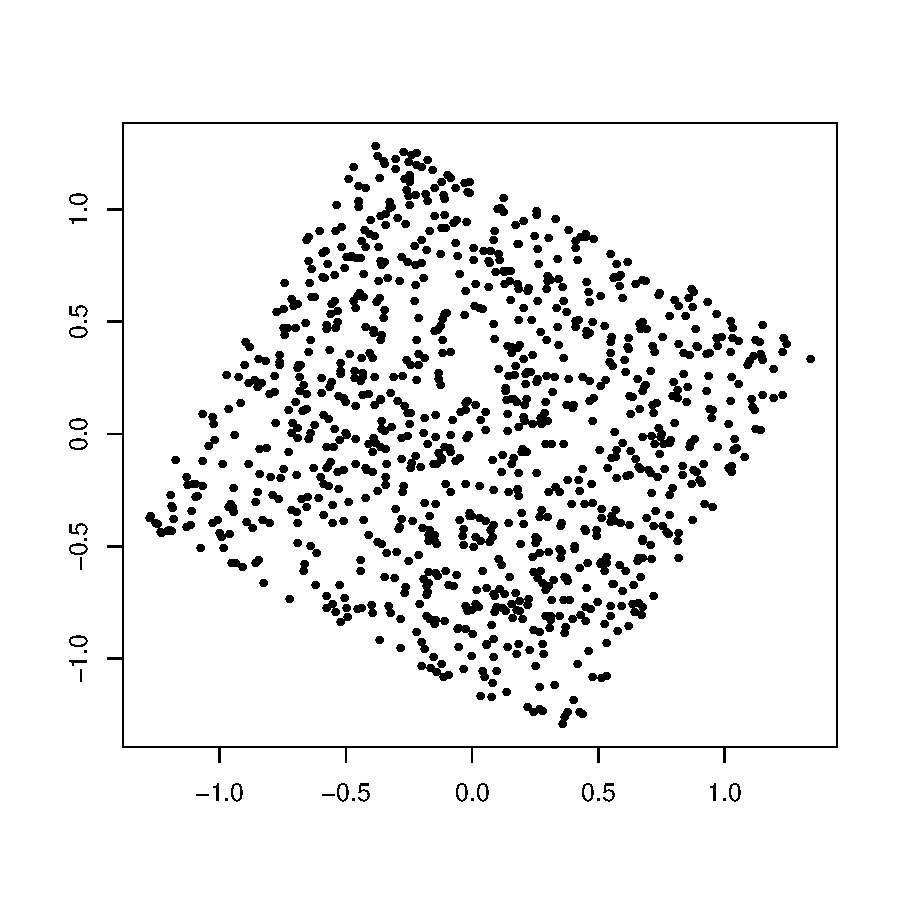
\includegraphics[scale=0.45]{ica-i.pdf}
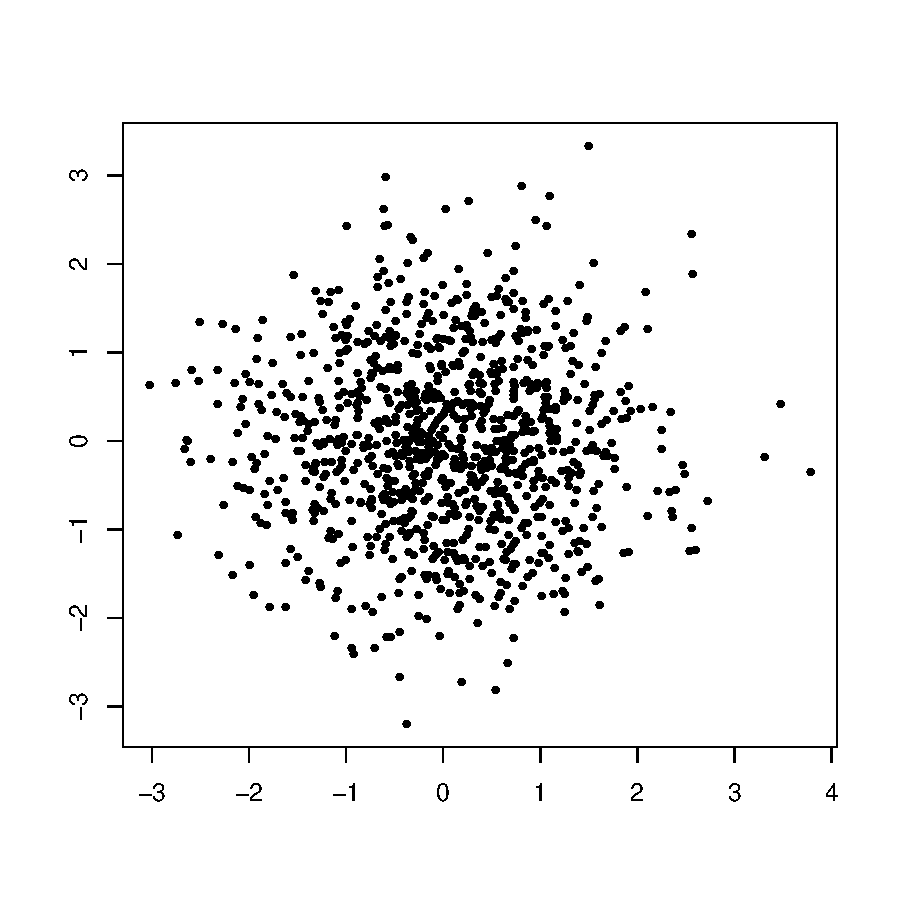
\includegraphics[scale=0.45]{ica-ii.pdf}
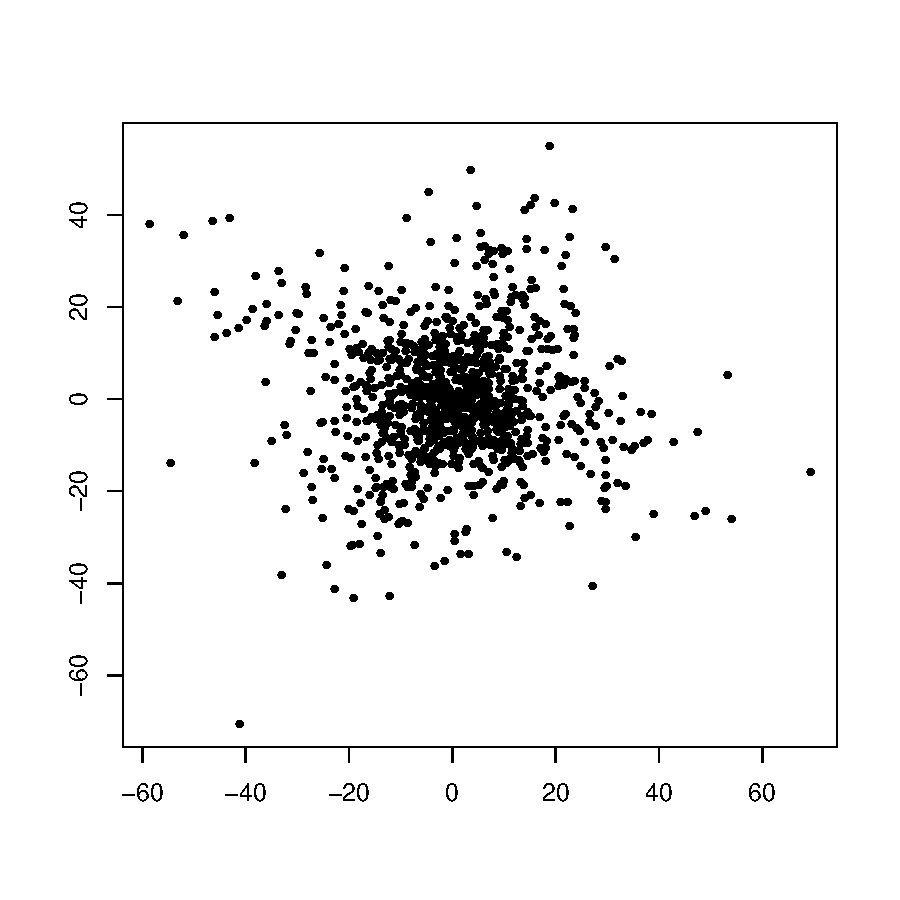
\includegraphics[scale=0.45]{ica-iii.pdf}
\end{center}\vspace*{-1cm}

It is possible to recover the translation and rotation only if independent components are sufficiently different form the normal distribution.  


\end{document}